% !Mode:: "TeX:UTF-8"

\chapter{使用矢量处理器对FDTD进行加速}

在本章中,我们以二维TM波为例来展示使用矢量处理器的加速方案。

\section{矢量处理器和数据并行}

在实际中常常会有对多个数据执行相同的操作,例如两个向量的内积,称之为矢量操作。对单个数据的操作称为标量操作。需要注意的是,这里的矢量仅仅说明数据是多个,而非是指代物理上有大小和方向的量。此处与之对应的标量是指单个数据,矢量和标量侧重的是数据数量的单数与复数,它们各自的简化结构示意图如图\ref{ch3:vectorprocessor}所示。数据并行就是对多个数据同时执行相同的操作,经典的使用数据并行的领域就是多媒体应用。矢量处理器的发展就是为了处理数据并行。

\begin{figure}[hp]
\centering
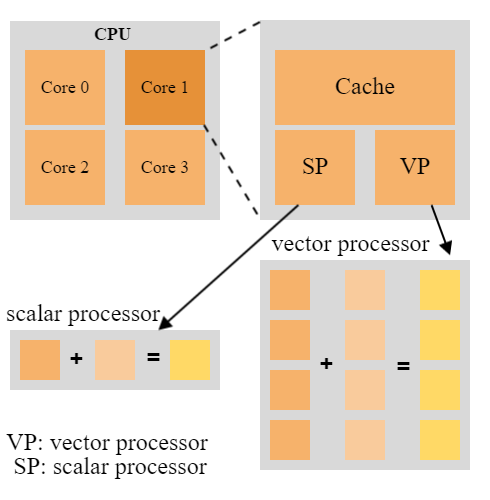
\includegraphics[width=0.7\linewidth]{pics/vectorprocessor}
\caption{矢量处理器与标量处理器}
\label{ch3:vectorprocessor}
\end{figure}


矢量处理器是可以利用指令操作矢量的中央处理单元。在使用时,使用指令让矢量处理器读入一个或多个经过打包(packed)的多个数据形成的一维数据列,然后使用指令让矢量处理器对这一个或者多个矢量的对应分量之间同时完成相同的操作,然后使用指令将计算结果返回内存中。

在使用矢量处理器计算的时候有一个和使用标量处理器很不同的地方在于数据的读入。在使用标量处理器的时候,由于每次只用从内存中读入单个数据,对单个数据 CPU 都会自动的处理好数据在内存中的对齐问题,所以不需要使用者有额外注意的事项,只要获得该数据的地址后直接读取即可。矢量处理器则不同,每次读入数据都需要读入连续的多个数据。这多个数据需要使用者在分配内存的时候显式的在内存中对齐,否则在读入数据时会消耗大量的资源。虽然只要数据是在内存中连续的,即使不对齐也可以读入到适量操作器中。但是即使是最优情况下非对齐的读入速度仍然比对齐情况慢了4.5倍。

\section{使用矢量处理器的FDTD加速原理}

以 TM 波为例。根据第二章可以得到$H_x$,$H_y$,$E_z$三个场分量的 FDTD 离散格式方程:
\begin{equation}\label{ch3: hx}
H^{n+\frac{1}{2}}_{x}\left(i,j+\frac{1}{2}\right)=H^{n-\frac{1}{2}}_{x}\left(i,j+\frac{1}{2}\right)+
\frac{\Delta t}{\mu}\left(
\frac{E^n_z(i,j)-E^n_z(i,j+1)}{\Delta y}
\right)
\end{equation}
\begin{equation}
H^{n+\frac{1}{2}}_{y}\left(i+\frac{1}{2},j\right)=H^{n-\frac{1}{2}}_{y}\left(i+\frac{1}{2},j\right)+
\frac{\Delta t}{\mu}\left(
\frac{E^n_z(i+1,j)-E^n_z(i,j)}{\Delta x}
\right)
\end{equation}
\begin{equation}\label{ch3: ez}
\begin{split}
E^{n+1}_z(i,j)=&E_z^n(i,j)\\
&+\frac{\Delta t}{\epsilon}\left(
\frac{H_y^{n+1/2}(i+\frac{1}{2},j)-H_y^{n+1/2}(i-\frac{1}{2},j)}{\kappa_x \Delta x}\right.\\
&\left.-\frac{H_x^{n+1/2}(i,j+\frac{1}{2})-H_x^{n+1/2}(i,j-\frac{1}{2})}{\kappa_y \Delta y}
\right)
\end{split}
\end{equation}

接下来以简单的$3\times3$网格来直观的说明数据并行计算的原理。根据第二章的场分量在 Yee 元胞中的空间排布方法,得到在$3\times3$的 Yee 网格中,场分量的排布应如图\ref{ch3 fig:2d yee}所示。其中格子内的序号代表该节点的位置,序号的第一位代表$y$方向的位置,即所在行数,序号的第二位代表$x$方向的位置,即所在列数。

\begin{figure}[hp]
	\centering
	\def \xcells {7}
	\def \ycells {7}
	\def \cell {1.2}
	\begin{tikzpicture}
	%\draw (0,0) grid (\xcells,\ycells);
	%Ez
	\foreach \x in {0,1,2,3}{
		\foreach \y in {0,1,2,3}{
			\filldraw[yellow] (2*\y,2*\x) rectangle (2*\y+1,2*\x+1);
			\node at (2*\y+0.5,2*\x+0.5) {\x,\y};
		}	
	}
	%grid
	\foreach \x in {1,3,5}{
		\foreach \y in {1,3,5}{
			\filldraw[lightgray] (\x,\y) rectangle (\x+1,\y+1);
		}	
	}
	%Hy
	\foreach \x in {0,1,2,3}{
		\foreach \y in {0,1,2}{
			\filldraw[pink] (2*\x,2*\y+1) rectangle (2*\x+1,2*\y+2);
			\node at (2*\x+0.5,2*\y+1.5) {\y,\x};
		}	
	}
	%Hx
	\foreach \x in {0,1,2}{
		\foreach \y in {0,1,2,3}{
			\filldraw[cyan] (2*\x+1,2*\y) rectangle (2*\x+2,2*\y+1);
			\node at (2*\x+1.5,2*\y+0.5) {\y,\x};
		}	
	}
	\draw [-stealth] (0,0) -- (\xcells+1,0) node[right] {$x$};
	\draw [-stealth] (0,0) -- (0,\ycells+1) node[right] {$y$};
	
	\filldraw[cyan] ($(0,-2)$) rectangle ($(0,-2)+(\cell,\cell)$);
	\node at ($(0,-2)+0.5*(\cell,\cell)$) {$H_x$};
	
	\filldraw[pink] ($(\cell,-2)$) rectangle ($(\cell,-2)+(\cell,\cell)$);
	\node at ($(\cell,-2)+0.5*(\cell,\cell)$) {$H_y$};
	
	\filldraw[yellow] ($(2*\cell,-2)$) rectangle ($(2*\cell,-2)+(\cell,\cell)$);
	\node at ($(2*\cell,-2)+0.5*(\cell,\cell)$) {$E_z$};
	
	\filldraw[lightgray] ($(3*\cell,-2)$) rectangle ($(3*\cell,-2)+(\cell,\cell)$);
	\node [align=center] at ($(3*\cell,-2)+0.5*(\cell,\cell)$) {Yee\\网格};
	\end{tikzpicture}
	\caption{TM 波中各场分量的 Yee 网格排布模型}
	\label{ch3 fig:2d yee}
\end{figure}

传统的数据并行方法对图\ref{ch3 fig:2d old}中的排布做了修改,在$x$增加方向的边界处增加了一列作为计算辅助而并无实际意义$H_x$节点。现在,设在$x$、$y$方向的Yee网格个数分别为$N_x$、$N_y$,则各个场分量在各个方向的节点数目表\ref{ch3: old number}所示。

\begin{figure}
	\centering
	\def \xcells {7}
	\def \ycells {7}
	\def \cell {1.2}
	\begin{tikzpicture}
	%\draw (0,0) grid (\xcells,\ycells);
	%Ez
	\foreach \x in {0,1,2,3}{
		\foreach \y in {0,1,2,3}{
			\filldraw[yellow] (2*\y,2*\x) rectangle (2*\y+1,2*\x+1);
			\node at (2*\y+0.5,2*\x+0.5) {\x,\y};
		}	
	}
	%grid
	\foreach \x in {1,3,5}{
		\foreach \y in {1,3,5}{
			\filldraw[lightgray] (\x,\y) rectangle (\x+1,\y+1);
		}	
	}
	%Hy
	\foreach \x in {0,1,2,3}{
		\foreach \y in {0,1,2}{
			\filldraw[pink] (2*\x,2*\y+1) rectangle (2*\x+1,2*\y+2);
			\node at (2*\x+0.5,2*\y+1.5) {\y,\x};
		}	
	}
	%Hx
	\foreach \x in {0,1,2,3}{
		\foreach \y in {0,1,2}{
			\filldraw[cyan] (2*\x+1,2*\y) rectangle (2*\x+2,2*\y+1);
			\node at (2*\x+1.5,2*\y+0.5) {\y,\x};
		}	
	}
	\draw [-stealth] (0,0) -- (\xcells+2,0) node[right] {$x$};
	\draw [-stealth] (0,0) -- (0,\ycells+1) node[right] {$y$};
	
	\filldraw[cyan] ($(0,-2)$) rectangle ($(0,-2)+(\cell,\cell)$);
	\node at ($(0,-2)+0.5*(\cell,\cell)$) {$H_x$};
	
	\filldraw[pink] ($(\cell,-2)$) rectangle ($(\cell,-2)+(\cell,\cell)$);
	\node at ($(\cell,-2)+0.5*(\cell,\cell)$) {$H_y$};
	
	\filldraw[yellow] ($(2*\cell,-2)$) rectangle ($(2*\cell,-2)+(\cell,\cell)$);
	\node at ($(2*\cell,-2)+0.5*(\cell,\cell)$) {$E_z$};
	
	\filldraw[lightgray] ($(3*\cell,-2)$) rectangle ($(3*\cell,-2)+(\cell,\cell)$);
	\node [align=center] at ($(3*\cell,-2)+0.5*(\cell,\cell)$) {Yee\\网格};
	\end{tikzpicture}
	\caption{传统数据并行计算模型}
	\label{ch3 fig:2d old}
\end{figure}


\begin{table}[hp]
\centering
\caption{TM波中各场分量在各方向上的节点个数}
\label{ch3: old number}
\begin{tabular}{ccc}
	\toprule
	场分量 & $x$方向未知量个数 & $y$方向未知量个数\\
	
	\midrule
	$E_z$ & $N_x+1$ & $N_y+1$\\
	$H_x$ & $N_x+1$ & $N_y$\\
	$H_y$ & $N_x+1$ & $N_y$\\
	\bottomrule
\end{tabular}
\end{table}

在计算时,首先我们使用指令分别为三个场分量的各自相应大小的对齐的连续内存空间。在$3\times3$的例子中,为$E_z$分配存放16个浮点数的内存空间,为$H_x$和$H_y$ 各自分配存放12个浮点数的内存空间。我们设定各个场分量都是先在$x$方向增长然后在$y$方向增长的,即节点的序号中首先增长代表$x$方向的那一位。所以,以$E_z$\linebreak[4]的内存举例,该场分量的内存中保存的节点按顺序分别为$(0,0)\cdots(0,3),(1,0)\cdots$。

在计算场分量时,以计算$H_x$为例说明,在说明示意时,不指定具体的操作适量操作器的指令集。第一步,根据\eqref{ch3: hx},我们读入三个矢量。第一个矢量包含$H_x$从第一个节点开始的五个节点,即$H_x(0,0)$到$H_x(1,0)$,记为$V_{H_x}$。第二个矢量包含$E_z$的从第一个节点开始的五个节点,即$E_z(0,0)$到$E_z(1,0)$,记为$V_{E_z}^1$。第三个矢量包含$E_z$从第二个节点开始的五个节点,即$E_z(0,1)$到$E_z(1,1)$,记为$V_{E_z}^2$。第二步,根据\eqref{ch3: hx},我们用指令让$V_{E_z}^1$减去$V_{E_z}^2$。减法操作为$V_{E_z}^1$的各项分别减去$V_{E_z}^2$中各自的对应项,得到的结果记为矢量$V_{sub}$。然后矢量$V_{sub}$的各项乘以常数$\frac{\Delta t}{\mu\Delta x}$得到记为$V_{sub}^{'}$的结果矢量。接着用指令让$V_{sub}^{'}$和$V_{H_x}$相加,得到最终结果。全部过程如图\ref{ch3 fig:cmp}所示。

\begin{figure}[hp]
\centering
\def \yshift {-1}
\def \xshift {1}
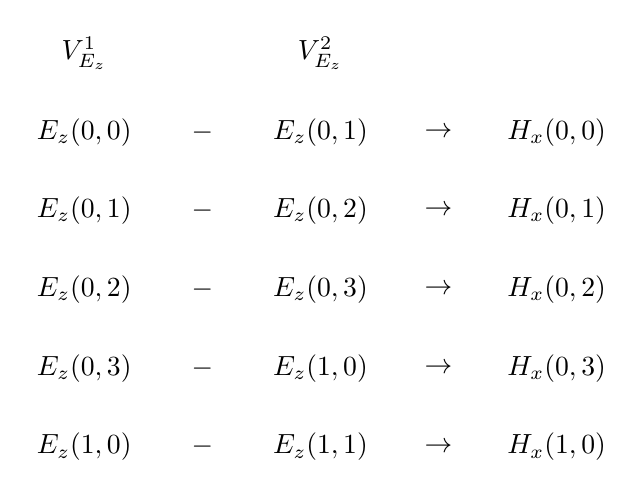
\begin{tikzpicture}

\node at (0,0) {$E_z(0,0)$};
\node at (0,\yshift) {$E_z(0,1)$};
\node at (0,2*\yshift) {$E_z(0,2)$};
\node at (0,3*\yshift) {$E_z(0,3)$};
\node at (0,4*\yshift) {$E_z(1,0)$};

\foreach \y in {0,1,2,3,4}{
	\node at (\xshift,\y*\yshift) {$-$};	
}

\node at (2*\xshift,0) {$E_z(0,1)$};
\node at (2*\xshift,\yshift) {$E_z(0,2)$};
\node at (2*\xshift,2*\yshift) {$E_z(0,3)$};
\node at (2*\xshift,3*\yshift) {$E_z(1,0)$};
\node at (2*\xshift,4*\yshift) {$E_z(1,1)$};

\foreach \y in {0,1,2,3,4}{
	\node at (3*\xshift,\y*\yshift) {$\rightarrow$};	
}

\node at (4*\xshift,0) {$H_x(0,0)$};
\node at (4*\xshift,\yshift) {$H_x(0,1)$};
\node at (4*\xshift,2*\yshift) {$H_x(0,2)$};
\node at (4*\xshift,3*\yshift) {$H_x(0,3)$};
\node at (4*\xshift,4*\yshift) {$H_x(1,0)$};

\node at (0,-\yshift) {$V_{E_z}^1$};
\node at (2*\xshift,-\yshift) {$V_{E_z}^2$};
\end{tikzpicture}
\caption{传统数据并行方案计算说明}
\label{ch3 fig:cmp}
\end{figure}


我们看到增添的作为辅助的节点$H_x(0,3)$使得矢量处理器在计算同一个场分量时,读入的矢量节点序号遵从相同的相对关系。在刚才的例子中,改关系就是读入的两组$E_z$节点的序号分别是和$H_x$相同以及序号的两位同时增加1。如果去掉这些辅助计算点,首先是在矢量处理器读入节点的时候需要有额外的计算所需读入节点的序号,其次是对于每行节点,都会有小于等于4个节点需要额外采取标量计算的方式进行计算。这两点大大增加了程序的复杂性和运行效率。

\section{一种新的数据并行FDTD计算模型}

上一节提到的传统的 Yee 网格可以适用于各种边界条件。但是对于某些边界条件,例如 Mur 吸收边界条件和 PEC 边界条件,我们可以进一步的改进计算中 Yee 网格中场分量的空间排布模型,减少场分量的节点数目,从而减少计算量。首先我们先来看 PEC 和 Mur 边界条件。

\paragraph{PEC截断边界条件} PEC 边界条件中,设置边界上的切向电场分量为0,即
\begin{equation}\label{ch3: pec}
E(K)=0
\end{equation}
其中$E(k)$代表边界处电场节点。这种边界条件称为截断边界条件。

\paragraph{Mur吸收边界条件} 使用 Mur 边界条件,就相当于在边界处涂吸波材料来吸收入射波,使得电磁波在边界处不会产生反射。考虑齐次波动方程的一维情形
\begin{equation}
\frac{\partial^2 u}{\partial x^2}-\frac{1}{c^2}\frac{\partial^2 u}{\partial t^2}=0
\end{equation}
解为
\begin{equation}
u(x,t)=A\exp[j(\omega t-k_x x)]
\end{equation}

设置$x=0$为左侧边界。由于仿真区域同时存在入射波和反射波,所以有
\begin{equation}
u(x,t)=A_{-}\exp[j(\omega t+k_x x)]+A_{+}\exp[j(\omega t-k_x x)]
\end{equation}
记该式右端第一项为$u_{-}$,第二项为$u_{+}$。对于边界$x=0$而言,$u_{-}$为入射波,$u_{+}$为反射波。如果让电磁波在边界处不产生反射,就要将反射波变为0。因此得到
\begin{equation}
\frac{\partial u}{\partial x}-\frac{1}{c}\frac{\partial u}{\partial t}=0
\end{equation}
对该式进行差分处理,得到
\begin{equation}\label{ch3: mur}
u^{n+1}(k)=u^n(k-1)+\frac{c\Delta t-\Delta z}{c\Delta t+\Delta z}[u^{n+1}(k-1)-u^n(k)]
\end{equation}
其中$u(k)$代表边界点,$u(k-1)$代表边界内最接近的相邻点。

根据两个边界条件的公式\eqref{ch3: pec}和\eqref{ch3: mur}来看,在计算边界处的电场节点时不需要其它场分量的节点或者只需要最邻近处相同场分量的节点。因此,我们可以对之前的 Yee 元胞场分量排布的计算模型进行简化,去除边界处电场节点之间的磁场节点,从而减少所需计算的节点数目,减少计算量。我们仍然以$3\times3$的规模的 Yee 网格为例来说明。新的计算模型如下图\ref{ch3 fig:2d new}所示。

\begin{figure}[hp]
	\centering
		\def \xcells {7}
		\def \ycells {7}
		\def \cell {1.2}
	\begin{tikzpicture}
	%\draw (0,0) grid (\xcells,\ycells);
	%Ez
	\foreach \x in {0,1,2,3}{
		\foreach \y in {0,1,2,3}{
			\filldraw[yellow] (2*\y,2*\x) rectangle (2*\y+1,2*\x+1);
			\node at (2*\y+0.5,2*\x+0.5) {\x,\y};
		}	
	}
	%grid
	\foreach \x in {1,3,5}{
		\foreach \y in {1,3,5}{
			\filldraw[lightgray] (\x,\y) rectangle (\x+1,\y+1);
		}	
	}
	%Hy
	\foreach \x in {0,1}{
		\foreach \y in {0,1,2}{
			\filldraw[pink] (2*\x+2,2*\y+1) rectangle (2*\x+3,2*\y+2);
			\node at (2*\x+2.5,2*\y+1.5) {\y,\x};
		}	
	}
	%Hx
	\foreach \x in {0,1,2}{
		\foreach \y in {0,1}{
			\filldraw[cyan] (2*\x+1,2*\y+2) rectangle (2*\x+2,2*\y+3);
			\node at (2*\x+1.5,2*\y+2.5) {\y,\x};
		}	
	}
	\draw [-stealth] (0,0) -- (\xcells+1,0) node[right] {$x$};
	\draw [-stealth] (0,0) -- (0,\ycells+1) node[right] {$y$};
	
	\filldraw[cyan] ($(0,-2)$) rectangle ($(0,-2)+(\cell,\cell)$);
	\node at ($(0,-2)+0.5*(\cell,\cell)$) {$H_x$};
	
	\filldraw[pink] ($(\cell,-2)$) rectangle ($(\cell,-2)+(\cell,\cell)$);
	\node at ($(\cell,-2)+0.5*(\cell,\cell)$) {$H_y$};
	
	\filldraw[yellow] ($(2*\cell,-2)$) rectangle ($(2*\cell,-2)+(\cell,\cell)$);
	\node at ($(2*\cell,-2)+0.5*(\cell,\cell)$) {$E_z$};
	
	\filldraw[lightgray] ($(3*\cell,-2)$) rectangle ($(3*\cell,-2)+(\cell,\cell)$);
	\node [align=center] at ($(3*\cell,-2)+0.5*(\cell,\cell)$) {Yee\\网格};
	\end{tikzpicture}
	\caption{改进的数据并行计算模型}
	\label{ch3 fig:2d new}
\end{figure}


从图中我们可以看到,处于 Yee 元胞所包含的范围之外的磁场节点全部被简化掉。现在的 Yee 网格计算模型中各个场分量在各方向上的节点数目如表\ref{ch3:new number}所示。同样设在$x$、$y$方向的 Yee 网格个数分别为$N_x$、$N_y$。

\begin{table}[hp]
	\centering
	\caption{TM 波中各场分量在新计算模型中各方向上的节点个数}
	\label{ch3:new number}
	\begin{tabular}{ccc}
		\toprule
		场分量 & $x$方向未知量个数 & $y$方向未知量个数\\
		
		\midrule
		$E_z$ & $N_x+1$ & $N_y+1$\\
		$H_x$ & $N_x$ & $N_y-1$\\
		$H_y$ & $N_x-1$ & $N_y$\\
		\bottomrule
	\end{tabular}
\end{table}

在计算时,和上一节中传统计算方法相同。首先我们使用指令分别为三个场分量的各自相应大小的对齐的连续内存空间。在$3\times3$的例子中,为$E_z$分配存放16个浮点数的内存空间,为$H_x$和$H_y$ 各自分配存放6个浮点数的内存空间。我们同样设定各个场分量都是先在$x$方向增长然后在$y$方向增长的,即节点的序号中首先增长代表$x$方向的那一位。

上一节中的计算模型中,由于$H_x$的辅助节点的存在,使得三个场分量各自的内存中所保存数据的位置和该数据对应的节点的序号是一致的,即在内存中第$m$个数据对应的节点分别是$E_z(m_y,m_x)$、$H_x(m_y,m_x)$和$H_y(m_y,m_x)$,三个节点的序号相同。但是在改进的计算模型中,该关系不再存在。这就导致矢量处理器在计算某个场分量时,读入的各个矢量中所包含的节点序号不再遵从相同的对应关系。同样以$H_x$的计算为例来说明。按照上一节中的操作,在计算$H_x$的钱四个节点时,矢量处理器需要读入三个矢量,分别是包含$H_x$从第一个节点开始的前四个节点,即$H_x(0,0)$到$H_x(1,0)$,记为$V_{H_x}$。第二个矢量是包含$E_z$第二行第一个节点开始的四个节点,即$E_z(1,0)$到$E_z(1,3)$,记为$V_{E_z}^1$。第三个矢量是包含$E_z$从第二行第二个节点开始的四个节点,即$E_z(1,1)$到$E_z(2,0)$,记为$V_{E_z}^2$。按照上一节所述的计算步骤,应该如图\ref{ch3:cmp}所示让$V_{E_z}^1$减去$V_{E_z}^2$。但是此时我们发现,两个矢量中前三个对应项的计算还正确,但是用来计算$H_x(1,0)$的第四项的减法就出现了错误。按照公式\eqref{ch3: hx},$H_x(1,0)$需要$E_z(2,1)$减去$E_z(2,0)$,但是实际上却是$E_z(2,0)$减去$E_z(1,3)$。

这个改变之处,导致了我们在计算时需要做两点调整,第一是在设计节点序号的地方,包括矢量处理器读入节点数据和对场分量的节点的计算,不能像传统方法一样将一种算法应用在整个场分量的内存所保存的数据上,而是必须将场分量分段处理,往往是按照 Yee 网格的行数分段,对于每一段分别应用某种算法。第二是在对场分量分段后每一段内存中的数据的处理,不能全部应用矢量处理器来计算。必须考虑到在每一段节点中,可能需要对该段前几个节点、中间部分节点和后几个节点分开处理,其中头尾处的节点需要使用标量处理器而非矢量处理器来计算。

\section{两种计算模型对比}

本文以二维 TM 波 FDTD 的 Mur 吸收边界条件为例来比较传统计算模型和改进计算模型的计算效率。我们分别对比使用传统计算模型和未使用数据并行的计算,以及在不同规模的仿真区域以及仿真时长下两种计算模型的区别。

程序的框架以调用树的形式展示,如图\ref{ch3 workflow:calltree}所示矩形框代表函数,箭头代表执行顺序。我们可以看到,程序分为两大部分,分别是对数据进行预处理的 $input$ 部分和对场分量节点进行计算的 \lstinline|compute| 部分。其中 \lstinline|compute| 又分为对磁场节点进行计算的 \lstinline|H_cmp| 部分和对电场节点进行计算的 \lstinline|E_cmp| 部分,以及进行辅助工作的其它函数。

\begin{figure}
	\centering
	\tikzstyle{box} = [rectangle, rounded corners, minimum width = 1cm,text centered, draw=black,align=center]
	\tikzstyle{arrow} = [thick,->,>=stealth]
	\begin{tikzpicture}
	\def \yshift {-1cm}
	\def \xshift {1.5cm}
	\node (main) [box] {\lstinline|main|};
	\node (input) [box,right of= main,yshift=-\yshift,xshift=\xshift] {\lstinline|input|};
	\node (compute) [box,right of=main,yshift=\yshift,xshift=\xshift] {\lstinline|compute|};
	\node (hcmp) [box,right of = compute,yshift=-\yshift,xshift=\xshift] {\lstinline|H_cmp|};
	\node (ecmp) [box,right of = compute,xshift=\xshift] {\lstinline|E_cmp|};
	\node (other) [box,right of = compute,yshift=\yshift,xshift=\xshift] {其它};
	
	\draw (main) --++(0.5*\xshift,0)--+(0,-\yshift)-- (input);
	\draw (main) --++(0.5*\xshift,0)--+(0,\yshift)-- (compute);
	\draw (compute) --++(\xshift,0)--+(0,-\yshift)-- (hcmp);
	\draw (compute) --++(\xshift,0)--+(0,\yshift)-- (other);
	\draw (compute) -- (ecmp);
	\draw [arrow] (input) -- (compute);
	\draw [arrow] (hcmp) -- (ecmp);
	\draw [arrow] (ecmp) -- (other);
	\end{tikzpicture}
	\caption{数据并行程序框架}
	\label{ch3 workflow:calltree}
\end{figure}

在分析时,我们采用 Visual Studio 的性能分析工具来收集样本的运行性能数据并进行分析。主要有两种分析方法,第一种是采样分析方法,第二种是检测分析方法。采样分析方法在每个 CPU 周期中断 CPU 并收集函数调用堆栈,对于不同类型的函数进行不同模式的样本数累加,从而收集分析运行期间应用程序所执行工作的相关统计数据。检测分析方法主要手机程序中函数调用的详细计时信息。该方法将捕获并检测每个函数的时间信息。时间信息主要包括两种,分别是:
\begin{description}
	\item[已用非独占时间]\quad 执行某函数或代码行所用的总时间。
	\item[已用独占时间]\quad 执行某函数体或代码行所用的时间。不包括执行该函数或代码行所调用的函数所用的时间。
\end{description}
所以,在样本程序中,\lstinline|main| 函数的已用非独占时间就代表了程序总花费时间,\lstinline|compute| 函数的已用非独占时间就代表了程序中计算场分量场点的时间花费。由于 \lstinline|H_cmp| 和 \lstinline|E_cmp| 函数没有调用函数,于是它们的已用独占时间和已用非独占时间相同,都是代表了执行一次该函数所用的时间。事实上,我们对这两个函数所关心的正是单次运行的时间。

为了保证各方法计算结果的准确性,各个样本的计算都运行5次去性能的平均值进行对比。编译时采取 Release 选项,这样能排除程序执行细节带来的对性能的影响,更能比较各个方案之间的性能差异。

计算环境为 Intel\textregistered Core\texttrademark i5-3210M 2.3GHz,4.00GB内存,操作系统为64-bit Windows 10。

下列各表展示了不同样本下性能对比结果。

\begin{table}[hp]
\centering
\begin{threeparttable}
	\caption{传统串行方案和改进计算模型方案性能比较}\label{ch3: data parallel or not}
	\begin{tabular}{cccc}
		\toprule
		\multirow{2}{2em}{函数}&\multicolumn{2}{c}{已用非独占时间(ms)} & \multirow{2}{11em}{使用数据并行所节约时间}\\
		\cline{2-3}
		& 不使用数据并行 & 改进计算模型 & \\ 
		
		\midrule
		\lstinline|main| & 10330.43 & 7835.78 & 24.15\% \\ 
		\lstinline|compute| & 10313.62 & 7819.76 & 24.18\%\\ 
		\lstinline|H_cmp|& 6.16 & 4.64 & 24.62\%\\ 
		\lstinline|E_cmp|& 4.10 & 3.13 &23.78\% \\
		\bottomrule
	\end{tabular} 
	\begin{tablenotes}
		\item[1] 仿真空间大小为$2000\times1000$个Yee网格。
		\item[2] 时间迭代次数为1000次。
	\end{tablenotes}
\end{threeparttable}
\end{table}

根据表\ref{ch3: data parallel or not}所示,我们可以看出在不适用数据并行的样本中 \lstinline|H_cmp| 和 \lstinline|E_cmp| 1000迭代的总占用时间分别约为6160ms和4100ms,两者之和为10260ms,占用\linebreak[4] \lstinline|main| 函数已用非独占时间的约99.3\%。同样,在使用数据并行的样本中该比例数值为99.2\%。这意味着这两个函数是程序的关键函数,所以如果不同的样本性能有有效差异,那么我们可以肯定的说差异就是因为这两个函数的不同导致的。在表\ref{ch3: data parallel or not}的比较中,我们可以看到使用数据并行可以节约大约24\%的时间,可以显著的缩短 FDTD 的计算耗时。

\begin{table}[hp]
\centering
\caption{传统数据并行方案和改进计算模型方案性能对比}\label{ch3: tradition or new}
\begin{threeparttable}
	\begin{tabular}{cccc}
		\toprule
		\multirow{2}{2em}{函数}&\multicolumn{2}{c}{已用非独占时间(ms)} & \multirow{2}{11em}{改进计算模型所节约时间}\\ 
		\cline{2-3}
		& 传统数据并行方案 & 改进计算模型 & \\ 
		
		\midrule
		\lstinline|main| & 4229.46 & 4082.64 & 3.47\% \\ 
		\lstinline|compute| & 4216.81 & 4070.73 & 3.46\%\\ 
		\lstinline|H_cmp|& 2.50 & 2.41 & 3.37\%\\ 
		\lstinline|E_cmp|& 1.68 & 1.62 & 3.57\% \\
		\bottomrule
	\end{tabular}
	\begin{tablenotes}
		\item[1] 仿真空间大小为$1000\times1000$个Yee网格。
		\item[2] 时间迭代次数为1000次。
	\end{tablenotes}
\end{threeparttable}
\end{table}

在表\ref{ch3: tradition or new}中我们可以看到,和传统数据并行方案相比,新的数据模型可以节省 FDTD 计算时间约为 3.45\%。基于上文对程序结构的分析,我们有理由排除掉程序细节的差异,得出改进后的计算模型优于旧方法的结论。我们可以看到,尽管删去一些磁场节点之后程序变得复杂,并且有一些节点的计算方式由之前的矢量处理器计算转换为了使用标量处理器计算,从而造成了部分性能的下降,但是减少计算节点而带来的性能增加可以完全抵消掉这一部分的性能下降,并且能在总体上提升性能。

\begin{table}[hp]
	\centering
	\begin{threeparttable}
	\caption{改进计算模型在不同仿真空间规模下的性能}\label{ch3: new, size}
		\begin{tabular}{cccc}
			\toprule
			\multirow{2}{2em}{函数}&\multicolumn{3}{c}{已用非独占时间(ms)}\\ 
			\cline{2-4}
			& $1000\times1000$ & $2000\times1000$ & $3000\times1000$\\ 
			
			\midrule
			\lstinline|main| & 4082.64 & 7835.78 & 11597.80 \\ 
			\lstinline|compute| & 4072.73 & 7819.76 & 11577.88\\ 
			\lstinline|H_cmp|& 2.412 & 4.64 & 6.87\\ 
			\lstinline|E_cmp|& 1.62 & 3.13 & 4.65 \\
			\bottomrule
		\end{tabular}
		\begin{tablenotes}
			\item[1] 时间迭代次数为1000次。
		\end{tablenotes}
	\end{threeparttable}
\end{table}

在表\ref{ch3: new, size}中我们可以看到,仿真计算所需的时间和仿真区域的规模成线性关系,时间复杂度为$O(n)$,所以改进后的模型可以用在实际应用中。这里所说的仿真区域的规模,是指 Yee 网格的数目。根据实验所收集的数据,当仿真规模增长了$n$倍的时候,时间消耗是之前的$0.92n+0.08$倍。

\begin{table}[hp]
	\centering
	\begin{threeparttable}
		\caption{改进计算模型在不同仿真时间规模下的性能}\label{ch3: new, time}
		\begin{tabular}{ccc}
			\toprule
			\multirow{2}{2em}{函数}&\multicolumn{2}{c}{已用非独占时间(ms)}\\ 
			\cline{2-3}
			& 1000次时间迭代 & 3000次时间迭代\\ 
			
			\midrule
			\lstinline|main| & 7835.78 & 23247.73 \\ 
			\lstinline|compute| & 7819.76 & 23230.83\\ 
			\lstinline|H_cmp|& 4.64 & 4.59\\ 
			\lstinline|E_cmp|& 3.13 & 3.10\\
			\bottomrule
		\end{tabular}
		\begin{tablenotes}
			\item[1] 空间规模是$2000\times1000$。
		\end{tablenotes}
	\end{threeparttable}
\end{table}

在表\ref{ch3: new, time}中,我们可以看到随着时间迭代次数的增加,程序的仿真时间也随之进行按照线性变化。不过我们也注意到,计算场分量的两个函数$H_cmp$和$E_cmp$的平均时间随着时间步的增加在下降。但是下降并不明显。时间迭代次数增长到了原来的300\%,时间减小幅度仅为1\%。我们推测这一部分的下降仅仅是由于增加了时间迭代次数之后,计算机能更为准确的进行内存命中,从而减少时间消耗,和算法是无关的。

\section{结论}

在本章中,我们以二维的TM波仿真为例,来展示说明了 FDTD 的数据并行计算中的一种新的计算模型。该模型主要是在传统计算模型的基础上修改了 PEC 截断边界条件和 Mur 吸收边界条件的情况下在边界处的磁场场分量点的分布。通过削减部分的磁场场分量计算点,在不影响计算结果的情况下,减少了仿真所需计算量,从而减少了仿真所需的计算之间。

通过对试验数据的分析,我们可以看到,使用数据并行可以大幅度的提升计算效率。而使用改进的数据并行计算模型之后,相比之前可以提升大约3.45\%的计算效率。这在大型 FDTD 仿真项目中会产生明显的区别。